\documentclass[varwidth=true, border=2pt]{standalone}

\usepackage{pgfplots}
\usepackage{tikz}

\begin{document}
	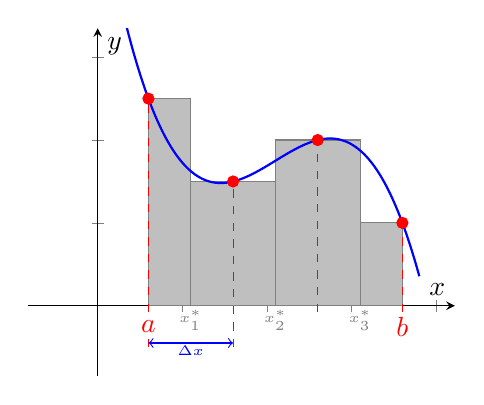
\begin{tikzpicture}
    \begin{axis}[
        legend pos=south east,
        axis x line=middle,
        axis y line=middle,
	xticklabels=\empty,
	yticklabels= \empty,
        grid = none ,
        width=7cm,
        height=6cm,
        grid style={dashed, gray!1},
        xmin=-2,     % start the diagram at this x-coordinate
        xmax=19,    % end   the diagram at this x-coordinate
        ymin=-1,     % start the diagram at this y-coordinate
        ymax= 6,   % end   the diagram at this y-coordinate
        xlabel=$x$,
        ylabel=$y$,
        enlargelimits=true,
        tension=0.08]

\filldraw[fill=lightgray, draw=gray] (axis cs: 3,0) rectangle (axis cs: 5.5,5);
\filldraw[fill=lightgray, draw=gray] (axis cs: 5.5,0) rectangle (axis cs: 10.5,3);
\filldraw[fill=lightgray, draw=gray] (axis cs: 10.5,0) rectangle (axis cs: 15.5,4);
\filldraw[fill=lightgray, draw=gray] (axis cs: 15.5,0) rectangle (axis cs: 18,2);


 \addplot[domain=1.25:19, blue, thick,samples=250] {-1/150*(x-8)*(x-13)*(x-18)+3/250*(x-3)*(x-13)*(x-18)-2/125*(x-3)*(x-8)*(x-18)+1/375*(x-3)*(x-8)*(x-13)}; % Parabola
  \addplot[red, only marks, mark=*] coordinates {(3,5)(8,3)(13,4)(18,2)};
  \draw [red,dashed] (axis cs: 3,-0.15) -- (axis cs: 3,5);
  \draw [red,dashed] (axis cs: 3,-1) -- (axis cs: 3,-0.7);
    \draw [red,dashed] (axis cs: 8,-1) -- (axis cs: 8,3);
     \draw [red,dashed] (axis cs: 13,-0.15) -- (axis cs: 13,4);
  \draw [red,dashed] (axis cs: 18,-0.15) -- (axis cs: 18,2);
  
  \draw [<->, blue] (axis cs: 3,-0.9) -- (axis cs: 8,-0.9);
      
%\filldraw[fill=lightgray, draw=gray] (axis cs: 0.5,0) rectangle (axis cs: 5.5,5);
	\node(a)[red] at (axis cs: 3,-0.5){$a$};
	\node(x1)[gray] at (axis cs: 5.5,-0.35){\tiny{$x_1^*$}};
	\node(xd)[blue] at (axis cs: 5.5,-1.1){\tiny{$\Delta x$}};
	\node(x2)[gray] at (axis cs: 10.5,-0.35){\tiny{$x_2^*$}};
	\node(x3)[gray] at (axis cs: 15.5,-0.35){\tiny{$x_3^*$}};
	\node(b)[red] at (axis cs: 18,-0.5){$b$};
%	\node(x1)[red] at (axis cs: 6,-0.5){$a \! +\! h$};
%	\node(x2)[red] at (axis cs: 10,-0.5){$a \! +\! 2h$};
%	\node(h1)[gray] at (axis cs: 4, 1){$h$};
%	\node(h2)[gray] at (axis cs: 8, 1){$h$};
    \end{axis}
\end{tikzpicture}
\end{document}